\section{Related Work}\label{sec:related_work}

\subsection{General Strategy}
Signature verification could be done by training a CNN to output whether or not the input image is of the chosen person.
However, this requires a new network to be trained for each person that the system needs to perform verification for.
Not only is it computationally very expensive to train such a system to perform verification for many people, but also requires a large number of images of the person's face for training.

Instead, a high-level representation of the image can be found that includes only the information needed to distinguish people.
This is effectively dimensionality reduction that preserves only the information that is important for identifying people.
The high-level representation is a vector in what is reffered to as a latent space.
(So, the dimensionality reduction should preserve/extract the structure of the person's face while discarding information about the background and the lighting conditions.)

\subsection{Handwriting Recognition} % remove if I'm out of space...
``In numerous situations, a pen together with paper or a small notepad is more convenient that a keyboard''\cite{handwriting_survey}.
Early research in automated recognition of handwriting was motiviated by the desire to allow humans to write conveniently and then parse that writing into data inside of a computer.

``On-line'' systems do this given the 2-D coordinates of the writer's pen as a function of time.% and require writing to be captured live by special electronic devices.
``Off-line'' systems only need images of the handwriting, so they are more broadly applicable\cite{handwriting_survey}.

Personal Digital Assistants (PDAs) incorporating on-line systems have been widely used commercially.
These systems have used rule-based, statistical, and implicit methods\cite{handwriting_survey}, espeacially Hidden Markov Models and even convolutional neural networks\cite{389575} (while LeCun's work was in its early stages\cite{mnist}).

None of these methods have been accurate enough to be used commercially on cursive writing\cite{handwriting_survey}.
As of 2000, on-line handwriting recognition was more accurate than off-line recognition because the chronological information is useful\cite{handwriting_survey}.
% However, off-line handwriting recognition is much more broadly applicable because it does not require a special device to capture the handwriting.
% Only a camera is needed to capture an image of the writing.
There have been several attempts made to recreate the temporal data from an image, but these have not been very successful\cite{handwriting_survey}.


% A bank might require an error of 1/ 100,000. ``Current systems are sill several orders of magnitude away''.

\subsection{MNIST/LeCun}
In 1998, LeCun famously tackled the problem of off-line handwritten digit recognition using convolutional neural networks\cite{mnist}.


\subsection{Contrastive Loss}
``The idea of mapping face images to low dimensional target spaces before comparison has a long history''
``Our approach is to build a trainable system that nonlinearly maps the raw images of faces to points in a low dimensional space so that the distance between these points is
small if the images belong to the same person and large otherwise. Learning the similarity metric is realized by training a network that consists of two identical convolutional
networks that share the same set of weights - a Siamese Architecture''
\begin{figure}[h]
    \begin{center}
        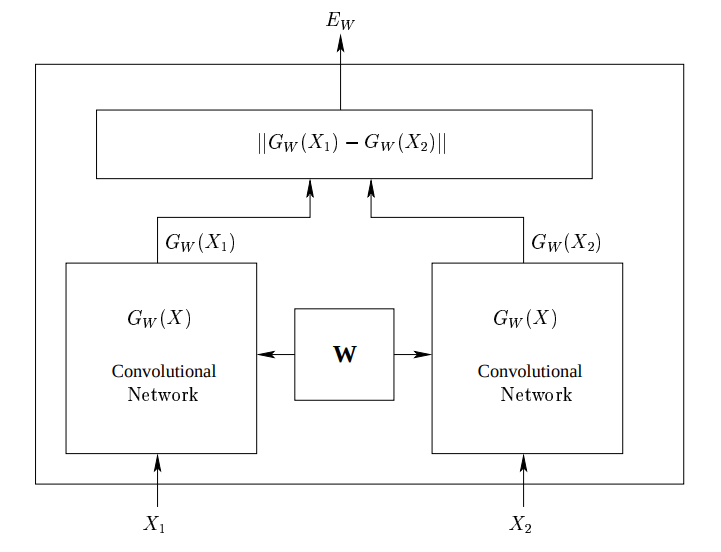
\includegraphics[width=0.8\linewidth]{siamese_architecture.png}
    \end{center}
    \caption{Siamese Architecture. (LeCun 2005)}
    \label{fig:siamese}
\end{figure}
I think LeCun proposed Contrastive Loss...\cite{LeCun}.
[Note: the partitioning and pairing of images is the same idea as SigNet.]
They did this on images of faces.

``A model is constructed of each subject by calculating the mean feature
vector and the variance-covariance matrix using the feature
vectors generated from the first five images of each subject.
The likelihood that a test image is genuine, $p_genuine$, is
found by evaluating the normal density of the test image on
the model of the concerned subject. The likelihood of a test
image being an impostor, $p_imposter$, is assumed to be a constant whose value is estimated by calculating the average $p_genuine$ value of all the impostor images of the concerned
subject. The probability that the given image is genuine is
given by P = $p_genuine$ / ($p_genuine$ + $p_imposter$)''
...so basically they assume that subjects/signers occupy a normal region in the latent space.

\subsection{Triplet Loss}
``FaceNet directly trains
its output to be a compact 128-D embedding using a triplet-based loss function based on LMNN [19]. Our triplets consist of two matching face thumbnails and a non-matching
face thumbnail and the loss aims to separate the positive pair
from the negative by a distance margin. The thumbnails are
tight crops of the face area, no 2D or 3D alignment, other
than scale and translation is performed.''
You could train a classifier and then take an intermediate layer to be a latent space, but this doesn't perform as well...
PCA can improve this, but an end-to-end network performs better.
\cite{face_net}

``The networks are trained by using a combination of classification and verification loss. The verification
loss is similar to the triplet loss we employ [12, 19], in that it
minimizes the L2-distance between faces of the same identity and enforces a margin between the distance of faces of
different identities. The main difference is that only pairs of
images are compared, whereas the triplet loss encourages a
relative distance constraint.''
``Although we did not directly compare to other losses,
e.g. the one using pairs of positives and negatives, as used
in [14] Eq. (2), we believe that the triplet loss is more suitable for face verification. The motivation is that the loss
from [14] encourages all faces of one identity to be projected onto a single point in the embedding space. The
triplet loss, however, tries to enforce a margin between each
pair of faces from one person to all other faces. This allows the faces for one identity to live on a manifold, while
still enforcing the distance and thus discriminability to other
identities.''
When training, they don't use true negatives to adjust weights because the network already knows they are different and so the direction of the gradient is somewhat arbitrary...
[Maybe I should try that...]
They just use a cut off threshold for computing accuracy.
I couldn't find how they chose the threshold...
Part of the results of their paper is that they conclude that using 256-bit over 128-bit latent vectos doesn't really improve accuracy.

\subsection{asdf}
this paper (where FaceNet got triplet loss...) allows datapoints with the same label to live in multiple clusters:
https://proceedings.neurips.cc/paper/2005/file/a7f592cef8b130a6967a90617db5681b-Paper.pdf
Does FaceNet allow a subject/person to live in several clusters?
The FaceNet paper suggests that each person lives in a single cluster (they imply that and their verifyication strategy is just a distance threshold...)

\subsection{SigNet}
``Unlike conventional approaches that assign
binary similarity labels to pairs, Siamese network aims to bring
the output feature vectors closer for input pairs that are labelled
as similar, and push the feature vectors away if the input pairs
are dissimilar.''
Uses Contrastive Loss (from LeCun).
Uses 128-bit latent vectors inspired by FaceNet.

``We initialize the weights of the model according to the work
of Glorot and Bengio [20], and the biases equal to 0. We trained
the model using RMSprop for 20 epochs, using momentum rate
equal to 0.9, and mini batch size equal to 128.''

In the paper, SigNet achieves 100\% accuracy on the CEDAR dataset, which contains 
In the validation process, SigNet takes an image and outputs a latent vector.
First, a genuine signature is sent through the network.
Then, either another genuine or a forge is sent throught the network.
The resulting latent vectors are compared using Euclidean distance.
[have I described partitioning yet?]
After computing the latent vector distances for all image pairs in the validation set, the threshold that results in the best accuracy is picked.
This results in 100\% accuracy on the CEDAR dataset.

SigNet was largely inspired by the success of FaceNet.
I haven't seen the SigNet paper discuss why they didn't use triplet loss...

Yo, why does SigNet use contrastive loss instead of triplet loss?
    My guess is that Contrastive Loss is just easier to implement...
\cite{sig_net}
\cite{GitHub_sounakdey}
...and in python: \cite{GitHub_signet_pytorch}

``In this paper, we model an offline writer independent
signature verification task with a convolutional Siamese network.''\cite{sig_net}

\subsection{DeepFool}
\subsection{DEFENSE-GAN}

\subsection{FGSM}
Ian Goodfellow (famous for his development of GANs) proves in this paper (https://arxiv.org/pdf/1412.6572.pdf) that even linear models are susceptable to avasarial attacks consisting of minute pertubations if their dimensionality is large enough.

``Here out epsilon of .007 corresponds to the magnitude of the
smallest bit of an 8 bit image encoding after GoogLeNet's conversion to real numbers.''
[Basically, I'll use the same epsilon value...]
They also should that training on adversarial inputs improves the model's accuracy on adversarial inputs (making it less sussecptible to the FGSM attack).

`` However, noise
with zero mean and zero covariance is very inefficient at preventing adversarial examples. The
expected dot product between any reference vector and such a noise vector is zero. This means that
in many cases the noise will have essentially no effect rather than yielding a more difficult input.''
...this means that adding my noise shouldn't really fool SigNet.

They also discuss ``whether it is better to perturb the input or the hidden layers or both''

Not related but interesting: don't perturb the last hidden layer because there arne't any hidden layers in between it and the output layer to fix the pertebatioons (using  universal approximator theorem)

``An intriguing aspect of adversarial examples is that an example generated for one model is often
misclassified by other models, even when they have different architecures or were trained on disjoint training sets.''
